\documentclass[11pt]{amsbook}
\usepackage[turkish]{babel}

\usepackage{../Ceyhun}	
\usepackage{../amsTurkish}

\usepackage{graphicx}
\usepackage{lipsum}



\begin{document}
\hPage{202}
\begin{figure}[htb]
	\centering
	

	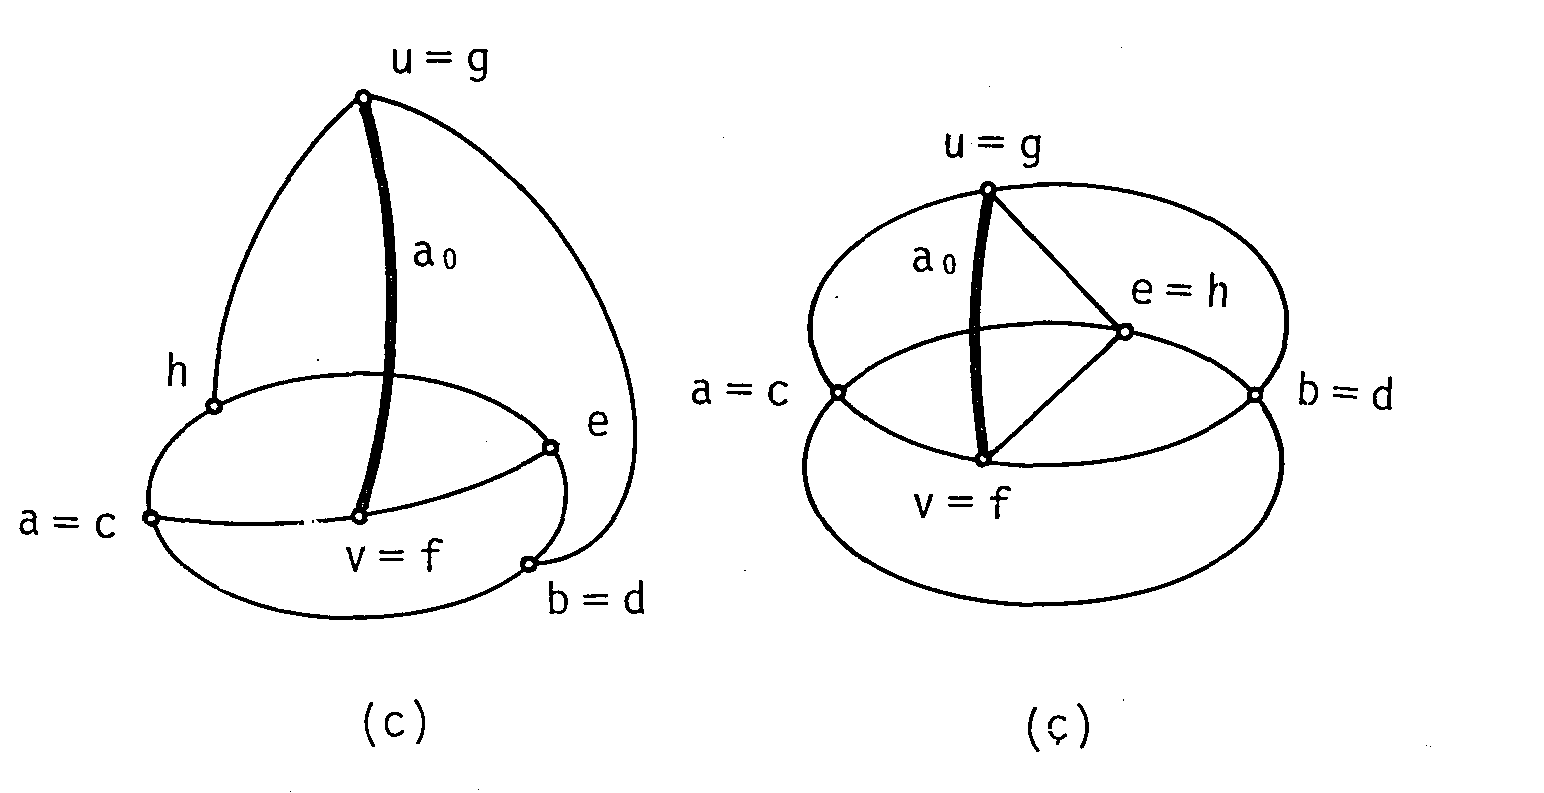
\includegraphics[keepaspectratio=true,scale=0.35]{images/ceyhun-202-fig01}
	\caption{$Y_{gh}$ yolunun konumuna göre, Durum 3 ün incelenmesi.}
	\label{fig:4.2.5}
	
\end{figure}
\\
İncelenecek bütün durumları tükettiğimiz için, 
Kuratowski Teoremi de tanıtlanmış olur.
\\
\\Kuratowski Teoremi, çizgelerin düzlemin ya da
eşanlamlı olarak yuvarlağın üzerine çizilebilmesi
için gerek ve yeter koşulu vermektedir. Düzleme 
çizilemeyen bir çizgeyi, yeterince sayıda
\textit{tutumak} eklenmiş bir yuvarlağın üzerine
çizebiliriz. Şekil~\ref{fig:4.2.6} da, üzerine bir ve iki
tutumak eklenmiş yuvarlaklara örnek verilmiştir.
Yuvarlağa çizilemeyen ve Şekil ~\ref{fig:4.2.7} de
gösterilen $D(7)$ ve $I(4,4)$ çizgelerini bir
\end{document}